In this section the implementation of the nested proof system is evaluated. The evaluation included measuring the system’s scalability and data handling capacity. This includes measuring the maximum number of inner proofs it can support within a given compiling time and assessing the volume of energy data it can process and verify. For the sake of simplicity and demonstrability only the proof generation time is evaluated here, as  the compilation and setup only need to be executed once.
The evaluation was conducted on a consumer laptop with a 1.6 GHz Dual-Core Intel Core i5 chip. 

The inner proof’s scalability was assessed by evaluating the impact of the amount of signatures that are verified within the proof while the outer proof's scalability was asses by the amount of inner proofs that that are provided. In both cases an exponential trend can be witnessed, as can be seen in Figure \ref{figure:number_of_innner}. This exponential growth in the proof’s computation time highlights ZoKrates scalability issues. While computational performance may improve with better hardware, the clear exponential trend indicates persistent scalability limitations. Furthermore, this limits the possibility of out- sourcing larger computations of the outer proof into the inner proofs. Adding more layers of proofs to split the computational load further is currently not supported for nesting in ZoKrates, which allows scalability improvement through nesting only to a small degree of two layers.

\begin{figure}[h]
\centering
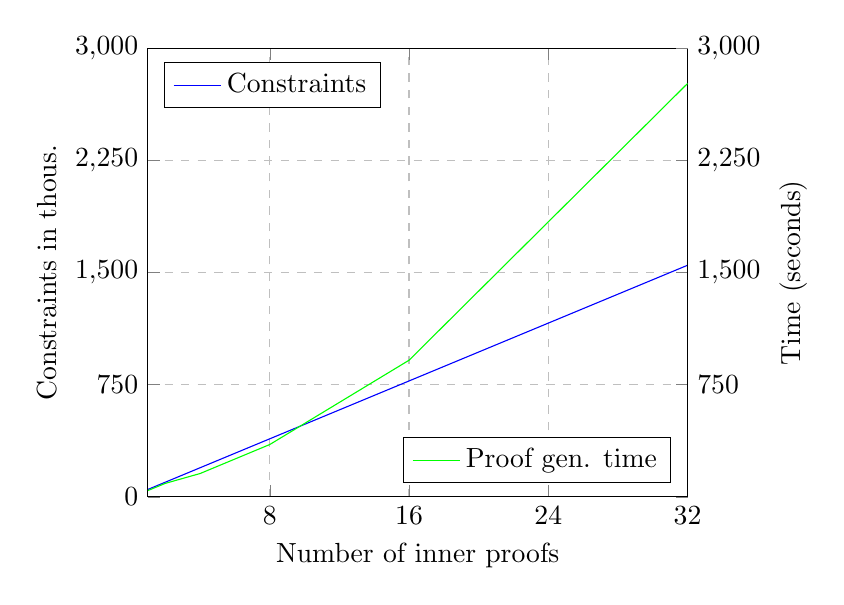
\begin{tikzpicture}
\begin{axis}[
    xlabel={Number of inner proofs},
    ylabel={Constraints in thous.},
    xmin=1, xmax=32,
    ymin=0, ymax=3000,
    xtick={8,16,24,32},
    ytick={0,750,1500,2250,3000},
    legend pos=north west,
    grid=major, % Enables major gridlines
    grid style=dashed,
]

\addplot[
    color=blue,
    mark=smooth,
    ]
    coordinates {
    (1,49.522)(2,97.912)(4,194.692)(8,388.252)(16,775.372)(32,1549.612)
    };
    \addlegendentry{Constraints}

\end{axis}

\begin{axis}[
    axis y line*=right,
    axis x line=none,
    xmin=1, xmax=32,
    ymin=0, ymax=3000,
    ylabel={Time (seconds)},
    ytick={750,1500,2250,3000},
    legend pos=south east,
]

\addplot[
    color=green,
    mark=smooth,
    ]
    coordinates {
    (1,42)(2,90)(4,156)(8,350)(16,914)(32,2766)
    };
    \addlegendentry{Proof gen. time}

\end{axis}
\end{tikzpicture}

\caption{Comparison of constraints and proof generation time for various numbers of inner proofs}
\label{figure:number_of_innner}
\end{figure}

However, as our evaluation was conducted merely up to 32 inner proofs or and signatures, we estimate the proof generation time for a higher number of inner proofs.   

Eberhardt et al. \cite{Netting} aimed for a proof generation time under 15 minutes for their netting proof with ZoKrates. However, in their system, the netting algorithm and proof generation require a more frequent execution. In contrast, the system proposed in this thesis needs to be executed less frequent. Assuming that the local utility has no hardware restrictions, unlike the smart meters or households, the proof generation time can extend multiple hours or even days. 

From 16 to 32 inner proofs, the base \( a \) of the proof generation time is 2.6 and increases for 1.16 each doubling of inner proofs, as observed from eight to 16 and 16 to 32. Assuming that the growth factor of \( a \) does not change, we can estimate the proof generation time (in seconds) for a given amount of inner proofs. We therefore modified the core formula for exponential growth , \( y = a^x \), for a scenario with a doubling of \( x \) and with a multiplicative increase of \( y \). In doing so logarithms are applied to convert the multiplicative relationships into additive ones, which can then be modelled through exponents. As the exponential growth does not start at \( x = 0 \), the formula is adjusted to account for an arbitrary starting point. Here, \( x \) represents the number of inner proofs, while \( y \) represents the proof generation time of the outer proof and \( y_0 \) represent the outer proof's generation time for the starting point \( x_0 = 32\), which is the maximum extent of my evaluation's computation.
 

\[
y = y_0 \cdot a^{\log_2\left(\frac{x}{x_0}\right)}
\]

\[
9709 = 2766 \cdot 3,51^{\log_2\left(\frac{64}{32}\right)}
\]

\[
45864 = 2766 \cdot 4,07^{\log_2\left(\frac{128}{32}\right)}
\]



With around 43 inner proofs, a proof generation time of approximately one hour is reached. The witness generation time accounts on top of that for about 10 to 20 percent of the proof generation time. Therefore, in realistic numbers, even fewer inner proofs can be nested for a computation time of one hour. Three hours of proof generation time allow for 96 inner proofs, assuming that the growth factor of \( a \) does not accelerate. Figure \ref{figure:estim} illustrates the continuation of the exponential trend for the proof generation time based on the introduced calculation.

\begin{figure}[h]
\centering
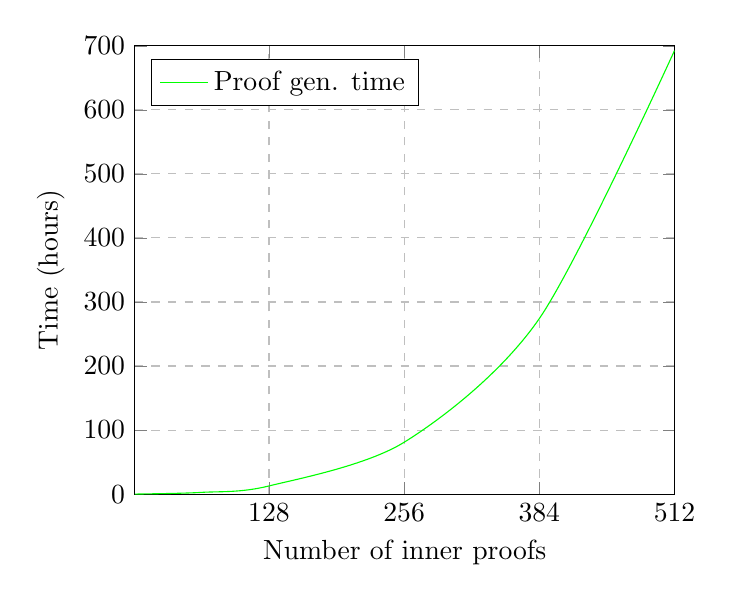
\begin{tikzpicture}
\begin{axis}[
    xlabel={Number of inner proofs},
    ylabel={Time (hours)},
    xmin=1, xmax=512,
    ymin=0, ymax=700,  % Adjusted to the max value provided in hours
    xtick={128,256,384,512},
    ytick={0,100,200,300,400,500,600,700},
    legend pos=north west,
    grid=major, % Enables major gridlines
    grid style=dashed,
]

\addplot[
    color=green,
    mark=none,
    smooth,
    ]
    coordinates {
    (1,42/3600)(2,90/3600)(64,9709/3600)(128,45864/3600)(256,291519/3600)(384,986877/3600)(512,2493276/3600)
    };
    \addlegendentry{Proof gen. time}

\end{axis}
\end{tikzpicture}

\caption{Estimating proof generation time per number of inner proofs}
\label{figure:estim}
\end{figure}


To better illustrate the requirements for a use case as presented in this paper, one district or neighbourhood within an eight-digit postal code area in Germany averages around 500 households \cite{ptvplz82210db}. The proof generation time for 512 households is approximately 29 days, assuming no other failures, such as memory constraints. Furthermore, the compiled circuit would have a size of around 264 GB and the proving key a size of around 51 GB, assuming a linear growth in those. This highlights ZoKrates scalability limits again, as such a system implemented in ZoKrates may accommodate only smaller communities and neighbourhoods.